

\chapter*{Eigenständigkeitserklärung}

Hiermit erkläre ich, dass ich die vorliegende Arbeit selbstständig angefertigt und keine anderen als die
angegebenen Hilfsmittel verwendet habe. Sämtliche verwendeten Textausschnitte, Zitate oder Inhalte anderer
Verfasser wurden ausdrücklich als solche gekennzeichnet.

\vskip 1cm


Wolfenschiessen, den 8. Juni 2018

\vskip 1.5cm

Daniel Zimmermann
\ihead[\sffamily \flushleft \sffamily BAT Schlussbericht\\  \small Eigenständigkeitserklärung]{\sffamily \flushleft \sffamily BAT Schlussbericht\\  \small Eigenständigkeitserklärung}	
\ofoot[]{}
%Anderungshistorie
\newpage
\ihead[]{\sffamily \flushleft \sffamily BAT Schlussbericht\\  \small Abstract}
%Titel ohne Nummerierung
\chapter*{Abstract}
\label{chap:abstract_englisch}
This documentation is the result of the bachelor thesis PIR Human Detector at the Lucerne School of Engineering and Architecture for the industry partner Schindler Aufzüge AG.

For maintenance and diagnostic purposes, the presence of persons in elevator cabins should be detected. Among other things, sensors that detect the thermal radiation are available for this purpose. In the context of the work, it should therefore be clarified to what extent passive infrared imaging sensors (PIR) are suitable for use in a elevator. 

A state-of-the-art PIR sensor is available for this purpose. The Panasonic Grid-Eye AMG8834 sensor offers only 8x8 pixels and measures the surface temperature in a limited field of view.  

In order to assess the suitability of the sensor, not only the physical and geometric properties are analysed, but also all sources of interference and influencing factors are determined. Several test procedures and measurement setups are used to identify and rate a wide variety of influencing factors. The analysis shows that the ambient temperature, the size of the person to be measured and the type of clothing play an important role in human detection. Built-in light sources, reflections and emissions of the surrounding materials are determined as sources of interference.  

In a further step, a neural network is created using machine learning. With the neural network and previously prepared data sets, it is possible to rate the quality of the measuring principle. The person detection is only carried out with zero to four persons, as the sensor characteristics in the measuring range haven't the resolution for more. 

The suitability of passive infrared sensors in elevators could be successfully verified with this bachelor thesis. But the quality depends on a few restriction, which are described in this document. An evaluation master and corresponding recommendations offer the possibility for further investigations. It also includes a few advices and feedbacks. 


\chapter*{Kurzbeschrieb}
\label{chap:abstract_german}
Diese Dokumentation ist das Ergebnis der Bachelorarbeit PIR Personendetektor an der Hochschule Luzern Technik \& Architektur für den Industriepartner Schindler Aufzüge AG. 

Für Wartungs- und Diagnosezwecke soll die Anwesenheit von Personen in Aufzugskabinen erfasst werden. Dazu bieten sich unter anderem Sensoren, welche die thermischen Strahlung detektieren. Im Rahmen der Arbeit soll daher geklärt werden, inwieweit sich bildgebende passiv Infrarotsensoren (PIR) für den Einsatzbereich in einem Personenaufzug eignen. 

Dafür steht ein State-of-the-Art PIR-Sensor zur Verfügung. Der verwendete Sensor Panasonic Grid-Eye AMG8834 bietet lediglich 8x8 Pixel und misst die Oberflächentemperatur in einem begrenzten Blickfeld.  

Um die Eignung des Sensors zu beurteilen, werden neben der Analyse der physikalischen und geometrischen Eigenschaften, vor allem auch Störquellen und Einflussfaktoren ermittelt. In mehreren Testdurchführungen und Messaufbauten werden verschiedenste Einflussfaktoren identifiziert und beurteilt. Bei der Analyse stellt sich heraus, dass bei der thermischen Personenerkennung hauptsächlich die Umgebungstemperatur, die Größe der zu messenden Person, sowie die Bekleidungsform eine bedeutende Rolle spielen. Als Störquellen werden Luftströme, sowie Reflexionen und Emissionen der umgebenden Materialien ermittelt.  

In einem weiteren Schritt wird auf der Basis des maschinellen Lernens und eigens erstellten Datensätzen ein neuronales Netzwerk implementiert, welches die Qualität der Personenerkennung wiedergibt. Dabei wird die richtige Detektion von null bis vier Personen ausgewertet, da die Sensoreigenschaften im Messbereich nicht mehr zulassen. 

Die Eignung von passiv Infrarotsensoren in Personenaufzügen konnte mit dieser Arbeit unter entsprechenden Einschränkungen, welche im Dokument ausführlich erläutert werden, erfolgreich verifiziert werden.
Ein Bewertungsraster und entsprechende Empfehlungen geben Auskunft über Schwachstellen des Messprinzips. Schlussendlich bieten offene Punkte die Möglichkeit für weitere Untersuchungen.   






%Inhaltsverzeichnis Dokumentation
\newpage
\ihead[\sffamily \flushleft \sffamily BAT Schlussbericht\\  \small Inhaltsverzeichnis]{\sffamily \flushleft \sffamily BAT Schlussbericht\\  \small Inhaltsverzeichnis}
\tableofcontents



%% Glossar
\newpage
\chapter*{Abkürzungverzeichnis}\addcontentsline{toc}{section}{Abkürzungsverzeichnis}
\begin{acronym}[LAMS aaaaaaaaa]

\acro{ASIC}{Anwendungsspezifische integrierte Schaltung}
\acroextra{eine elektronische Schaltung, die als integrierter Schaltkreis realisiert wurde}
\acro{IoT}{Internet of Things}			\\ \acroextra{Technologien einer globalen Infrastruktur der Informationsgesellschaften}
\acro{MEMS}{Mikroelektromechanisches System} 	\\ \acroextra{Technologien einer globalen Infrastruktur der Informationsgesellschaften}
\acro{PIR}{passiv Infrarot Sensoren}	\\ \acroextra{Sensorik}
\acro{FOV}{Field Of View}             	\\ \acroextra{bezeichnet den Bereich im Bildwinkel eines optischen Sensors}
\acro{NETD}{Rauschäquivalente Temperaturdifferenz} \\
{Ein Maß für das Bildrauschen einer Infrarotkamera}
 


\end{acronym} 

\ihead[\sffamily \flushleft \sffamily BAT Schlussbericht\\  \small Abkürzungsverzeichnis]{\sffamily \flushleft \sffamily BAT Schlussbericht\\  \small Abkürzungsverzeichnis}


%% Abbildungen
\newpage
\ihead[\sffamily \flushleft \sffamily BAT Schlussbericht\\  \small Abbildungen]{\sffamily \flushleft \sffamily BAT Schlussbericht\\  \small Abbildungen}
\listoffigures \addcontentsline{toc}{section}{Abbildungen}

%% TABELLEN
\newpage
\ihead[\sffamily \flushleft \sffamily BAT Schlussbericht\\  \small Tabellen]{\sffamily \flushleft \sffamily BAT Schlussbericht\\  \small Tabellen}
\listoftables \addcontentsline{toc}{section}{Tabellen}
%% EQUATUIN
\ihead[\sffamily \flushleft \sffamily BAT Schlussbericht\\  \small ]{\sffamily \flushleft \sffamily BAT Schlussbericht\\  \small Formeln}
\listofmyequations \addcontentsline{toc}{section}{Formeln} 
\newpage
\ihead[\sffamily \flushleft \sffamily BAT Schlussbericht\\  \small Literaturverzeichnis]{\sffamily \flushleft \sffamily BAT Schlussbericht\\  \small Literaturverzeichnis}
\printbibliography[ keyword={online}, title={Literaturverzeichnis}]\addcontentsline{toc}{section}{Literaturverzeichnis} 
\clearpage 


%Zielbestimmung
\ihead[]{\sffamily \flushleft \sffamily BAT Schlussbericht\\  \small \rightmark}
\newpage
\chapter{Einleitung}
\label{chap:Einleitung}


\label{sec:Ausgangssituation}
Durch den technologischen Wandel, den die Industrie 4.0 sowie \ac{IoT}  mit sich bringen, entstehen in verschiedensten Einsatzbereichen neue Möglichkeiten. Die Sensoren werden zunehmend kleiner, vernetzter und günstiger. Dazu stehen stetig schnellere Prozessoren und größere Speicherkapazitäten zur Verfügung, daher werden vermehrt auch in alltäglichen Situation intelligente Systeme eingesetzt. 

Für Wartungs- und Diagnosezwecke von Personenaufzügen bieten solche intelligente Systeme ein bedeutendes Potential. Durch die ortsunabhängige Kommunikation von übergreifenden Netzwerken und der Echtzeitverarbeitung bieten solche Messeinheiten Alternativen zu teuren Servicegängen. Mittels ständiger Überwachung und Fernwartung können Probleme frühzeitig erkannt und behoben werden. Die Anforderungen an eine solche Messeinheit hängt jedoch stark von Einsatzort ab. Dabei spielen Langzeiteinsatz, Zuverlässigkeit, Flexibilität, sowie auch der Energieverbrauch eine bedeutende Rolle.

Ein relevantes Messobjekt für eine solche Messeinheit ist unter anderem die Anzahl Personen innerhalb eines Aufzugs. Da übliche Überwachungskameras und bildgebende TOF-Sensoren teuer sind und einen bedeutenden Energiebedarf besitzen, stellt sich in diesem Bereich die Frage nach einer Alternative.

\section{Aufgabenstellung}
\label{chap:Aufgabenstellung}
An diesem Punkt setzt nun die Aufgabenstellung dieser Bachelorarbeit an. Es soll die Eignung von \ac{PIR} für eine solche Messeinheit geprüft werden. Dabei wird ein typischer bildgebender PIR-Sensor in möglichst breiter und wegweisender Form beurteilt. Es wird dabei der State-Of-the-Art Sensor AMG8834 von Panasonic verwendet. Mit diesem sollen in einer ersten Phase grundlegende Grenzen und Eigenheiten dieses passiven Messprinzips erarbeitet werden. In einem weiteren Schritt soll auf der Grundlage von Messresultaten und Testdurchführungen ein prototypische Messeinheit und ein Auswertealgorithmus entwickelt werden, mit welchem sich Personen innerhalb des Messbereichs detektieren lassen. Abschließend wird das Messprinzip beurteilt und eine Empfehlung für die Weiterführung gebildet. 

\section{Ziele}
\label{sec:Einleitung}
In erster Linie soll mit dieser Arbeit die Fragestellung geklärt werden, ob sich bildgebende \ac{PIR} für die Personendetektion in Personenaufzügen eignen. Ziel dieser Bachelorarbeit ist es, einen breiten und fundierten Katalog über die Möglichkeiten und Grenzen des PIR-Sensors zu liefern. Diese Bachelorarbeit begrenzt sich auf die Analyse des Messprinzips von bildgebenden PIR Sensoren. Es werden keine Vergleiche mit anderen Sensorarten durchgeführt.

\section {Methodik}
\label{sec:Methodik}
Die gesamte Arbeit wurde etappenweise gegliedert. Zuerst wurde einen Zeitraum für die Informationsbeschaffung definiert. Danach wiederholen sich Testphasen, Datenerfassungen und Auswertungen. Einzelne Testkonzepte geben Auskunft über die Testdurchführungen, sowie die entsprechenden Testspezifikationen. Für die Datenverarbeitung und Aufbereitung wird mittels Matlab und Python 3.5 programmiert.  Für den Auswertealgorithmus wird das Prinzip des maschinellen Lernens angewendet. Dafür steht die Open-Source-Library Tensorflow r1.7 von Google zur Verfügung.


Das Projektmanagement in Anhang \ref{AnhangA} - \ref{AnhangC} \todo{referenz} beinhaltet neben den detaillierten Projektplan auch die anfänglich definierten Meilensteine. Im detaillierten Projektplan sind neben den Tätigkeiten auch die zeitlichen Abschätzungen als Soll-/Ist-Vergleich angefügt. im Kapitel \ref{chap:Reflexion} werden zum Projektmanagement kurz Stellung genommen und grössere Differenzen kommentiert.



\ofoot[]{\pagemark}
\chapter{Informationsbeschaffung}
\label{chap:Informationsbeschaffung}
Dieses Kapitel bietet fundamentale physikalische Gegebenheiten, sowie die relevanten Eigenheiten des verwendeten \ac{PIR}-Sensors. Da es sich um eine bildgebendes Messprinzip handelt, werden des Weiteren geometrische Aspekte erläutert. Schlussendlich bietet dieses Kapitel auch nötige Informationen über das Messobjekt bzw. die Messumgebung geliefert.

\section{Grid-Eye AMG8834}
\label{sec:AMG8834}

Der verwendete Panasonic AMG8834 ist ein bildgebender \ac{MEMS}-Sensor, der mit insgesamt 64 temperaturempfindlichen Thermosäulenelementen ausgestattet ist. Diese sind als 8x8 Pixel-Matrix auf den Chip aufgebracht. In Abbildung \ref{fig:Explosionsdarstellung} ist der Aufbau des Sensors dargestellt.
 
\begin{figure}[H]
	\centering
	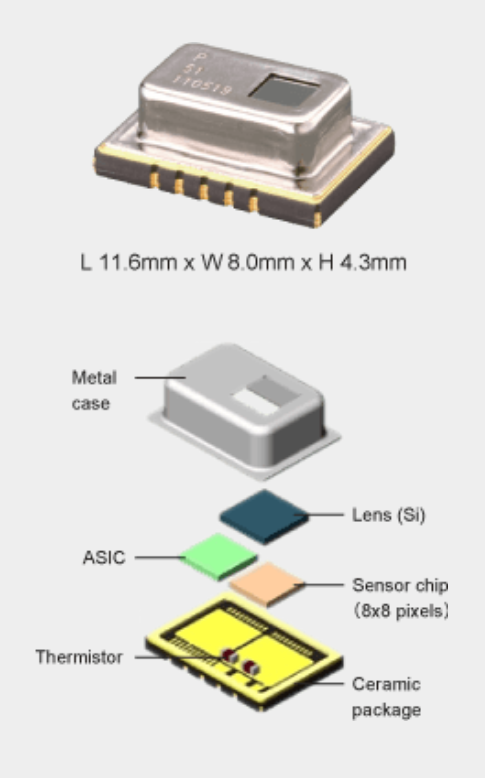
\includegraphics[width=0.3\textwidth]
	{fig/grid_eye_aufbau.PNG}
	\caption[Schema des AMG8834 Sensors]{Schema des AMG8834 Sensors} \protect\cite{AMG8834}
	\label{fig:Explosionsdarstellung}
\end{figure}
Die eintreffenden Infrarotwellen werden durch die Siliziumlinse, welche einen \ac{FOV} von 60$^\circ$ besitzt, gefiltert. Dabei durchdringen lediglich langwellige Infrarotstrahlungen mit den Wellenlängen 8-13 $\mu$m die Linse. Dies entspricht dem dritten atmosphärischen Fenster.

In Abbildung \ref{fig:SchemaAMG8834} ist das Prinzipschema des Sensors darstellt. Das Messprinzip des Sensors wird im Unterkapitel \ref{subsec:seebeck} detailliert erläutert. Die entstandene Thermospannung wird durch die \ac{ASIC} des \ac{MEMS}-Sensor verarbeitet. Das selektierte Thermospannung wird verstärkt, mit dem integrierten Thermistor verglichen und mit dem \ac{ADC} gewandelt. Durch die hohe interne Verstärkung besitzt der Sensor jedoch bei normalen Bedingungen\footnote[2]{Umgebungstemperatur 0-80 $^\circ$C bei Luftfeuchtigkeit 15-85\%} eine Genauigkeit von +/- 3°C. 

\begin{figure}[H]
	\centering
	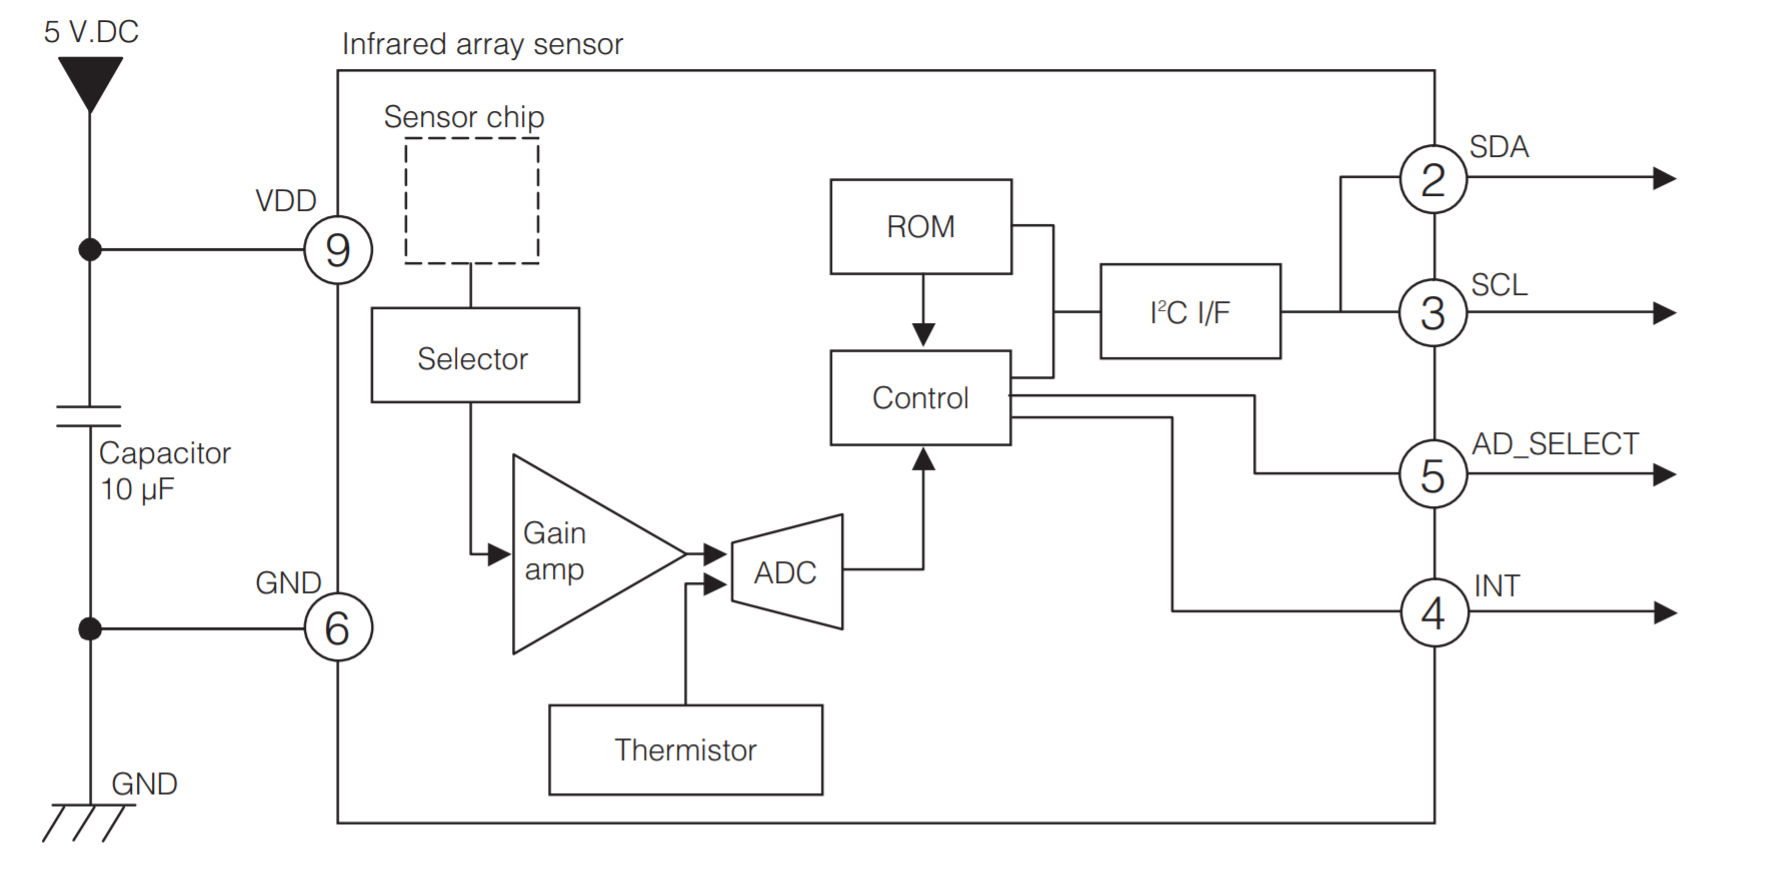
\includegraphics[width=0.75\textwidth]
	{fig/Circuit_AMG8834.PNG}
	\caption[Schema des AMG8834 Sensors]{Schema des AMG8834 Sensors} \protect\cite{AMG8834}
	\label{fig:SchemaAMG8834}
\end{figure}
 
Über die \ac{I2C} lassen sich die Werte der Thermoelemente und der Thermistoren je aus 2 Register auslesen. Die Messwerte werden alle 100 ms aktualisiert. Dabei werden lediglich 12 Bit pro Pixel für die Temperaturregister genutzt. Dies führt zu der kleinsten unterscheidbaren Größe von 0.25 $^\circ$C . Die Thermistorregister lassen sich mit der Auflösung von 0.625 $^\circ$C unterscheiden. In Abbildung \ref{fig:SchemaAMG8834} ist klar ersichtlich, dass die Umgebungstemperatur, bzw. die Temperatur, welche vom Thermistor gemessen wird direkten Einfluss auf die Pixelwerte besitzen. Variieren die Thermistorwerte aufgrund von Raumtemperaturschwankungen können die Pixelwerte dadurch bedeutende Abweichungen entstehen.

\section{Physikalische Aspekte}
\label{sec:Physik}
Dieser Abschnitt erläutert auf kurze und prägnante Weise, physikalischen Aspekte die dem Sensor zu Grunde liegen. Dies bietet die Grundlage für die Bestimmung der Störquellen und das Verhalten des Sensors bei entsprechenden äußeren Einwirkungen. Die Tabelle \ref{tab:Legende Physikalische Grössen} gibt die Bezeichnungen der nachfolgenden Formeln wieder.

\begin{table}[H]
	\centering
	\begin{tabular}{l|c|c}
		\rowcolor{gray} Grösse &  Bezeichnung  & Einheit \\
		\hline 
		Thermospannung &  $ U_{t}$ & $J$  \\ 
		\rowcolor{gray} Thermokraft P/N -Silizium  & $\alpha_{p},\alpha_{n}$ & $V/K$\\	
		Temperatur P/N -Silizium &  $T_{p},T_{n}$ & $V/K$ \\
		\rowcolor{gray}Wärmestrom &  $\dot{Q}$ & $J$  \\ 
		Emission & $\epsilon$ & $-$\\	
		\rowcolor{gray}Reflektion &  $\rho $ & $-$ \\
		Transmission & $\tau$ & $-$\\
		\rowcolor{gray}Absoprtion &  $\alpha$ & $-$  \\ 
		Strahlungsleistung & $\dot{Q}$ & $W$\\
		\rowcolor{gray}spektrale spezifische Ausstrahlung &  $M_{\lambda }$ & $W/sr$\footnote[3]{Steradiant: Messeinheit für den Raumwinkel} \\
		Planksches Wirkungsquantum &  $ h$ & Js \\ 
		\rowcolor{gray} Lichtgeschwindigkeit im Vakuum & $c $ & $ m/s$ \\ 
 		Stefan-Boltzmann-Konstante & $\sigma$ & $ W/m^2K^2 $ \\ 
	\end{tabular}
	\caption{Legende physikalische Grössen Konzeptzeichnungen}
	\label{tab:Legende Physikalische Grössen} 
\end{table} 


\subsection{Seebeck-Effekt}
\label{subsec:seebeck}
Die durch die konvexe Linse gesammelten Infrarotstrahlen verursachen auf den einzelnen Thermosäulenelemente (2), dass die Oberfläche erwärmt wird. Es entsteht zwischen der erwärmten, n-dotierten Siliziumschicht (4) und der kühleren p-dotierten Siliziumschicht (6) ein Temperaturgefälle.   

\begin{figure}[H]
	\centering
	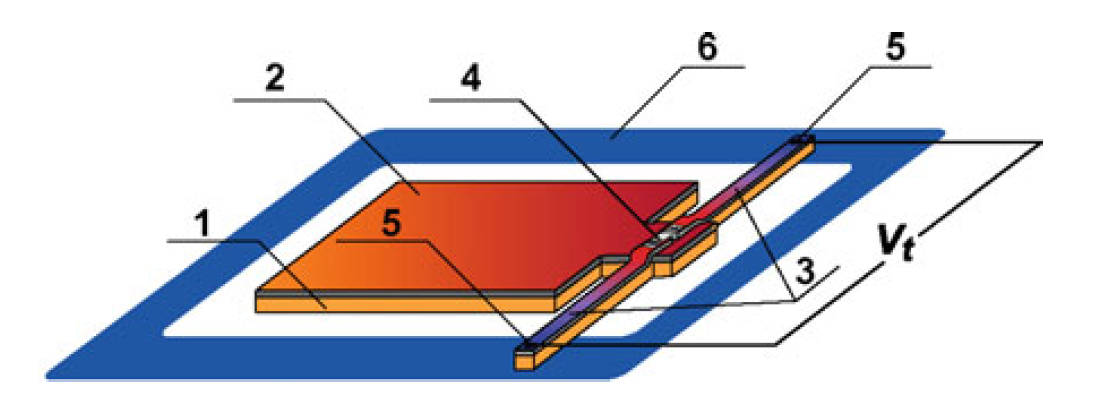
\includegraphics[width=0.6\textwidth]
	{fig/Mems_Thermopile.PNG}
	\caption[Aufbau Thermosäulenelement]{Aufbau Thermosäule} \protect\cite{AMG8834}
	\label{fig:AufbauThermo}
\end{figure}

\todo{Kotrolle Thermosäule} Durch die unterschiedlichen Thermokräfte (auch Seebeckkoeffizienten) der zwei Halbleitermaterialien entsteht ein Potentialunterschied, den man an den Punkten 3 und 5 abgreifen kann. Diese Spannung $U_{t}$ ist die Grundlage des Messprinzips und wird mit Formel \ref{eq1} \protect\cite{AMG8834} beschrieben.


\begin{equation}
\label{eq1}
U_{t} = (\alpha_{p} + \alpha_{n})*(T_{p}+T_{n})
\end{equation}
\begin{center}

\end{center}
\myequations{Seebeck-Effekt}


\subsection{Strahlungstheorie}
\label{subsec:Strahlungstheorie}
Das vorherige Unterkapitel erläutert die Funktion des Sensors als Infrarotempfänger. Nicht unwesentlich ist weiter die Betrachtung des Senders. Grundsätzlich gilt, jeder Körper, der eine Temperatur oberhalb des absoluten Nullpunkt aufweist, strahlt Wärmestrahlung im Infrarotbereich ab. 

Im Allgemein wird für die Betrachtung vom Plank'schen Strahlungsgesetz ausgegangen. Nach dieser gilt für eine spektrale spezifische Ausstrahlung eines Schwarzkörpers mit der Temperatur T folgende Formel \protect\cite{Thermoformeln}:

\begin{equation}
\label{eq2}
M_{\lambda } = \frac{2\pi h c^2 }{\lambda^5}*\frac{1}{e^\frac{hc}{\lambda k_{B} T}-1}
\end{equation}
\myequations{Plank'sches Strahlungsgesetz}

Wie in der Formel ersichtlich ist die Ausstrahlung eines schwarzen Körper mit 5. Potenz von der Wellenlänge und exponentiell von der Temperatur abhängig. Durch die Siliziumlinse des Sensors werden somit Störquellen, welche andere Wellenlängen aufweisen, gefiltert. Dies ist vor allem bei Lichtquellen ein relevante Eigenschaft.

Das Stefan-Boltzmann-Gesetz \protect\cite{Thermoformeln} gibt die Strahlungsintensität $\dot{Q}$ eines idealen Temperaturstrahlers an. Diese Formel bietet für die Anwendung die relevantesten Erkenntnisse.


\begin{equation}
\label{eq3}
\dot{Q} = \frac{\mathrm{d} Q}{\mathrm{d} t} = \epsilon *\sigma * A * T_{obj}^4
\end{equation}
\myequations{Wärmestrahlung }

\begin{figure}[H]
	\centering
	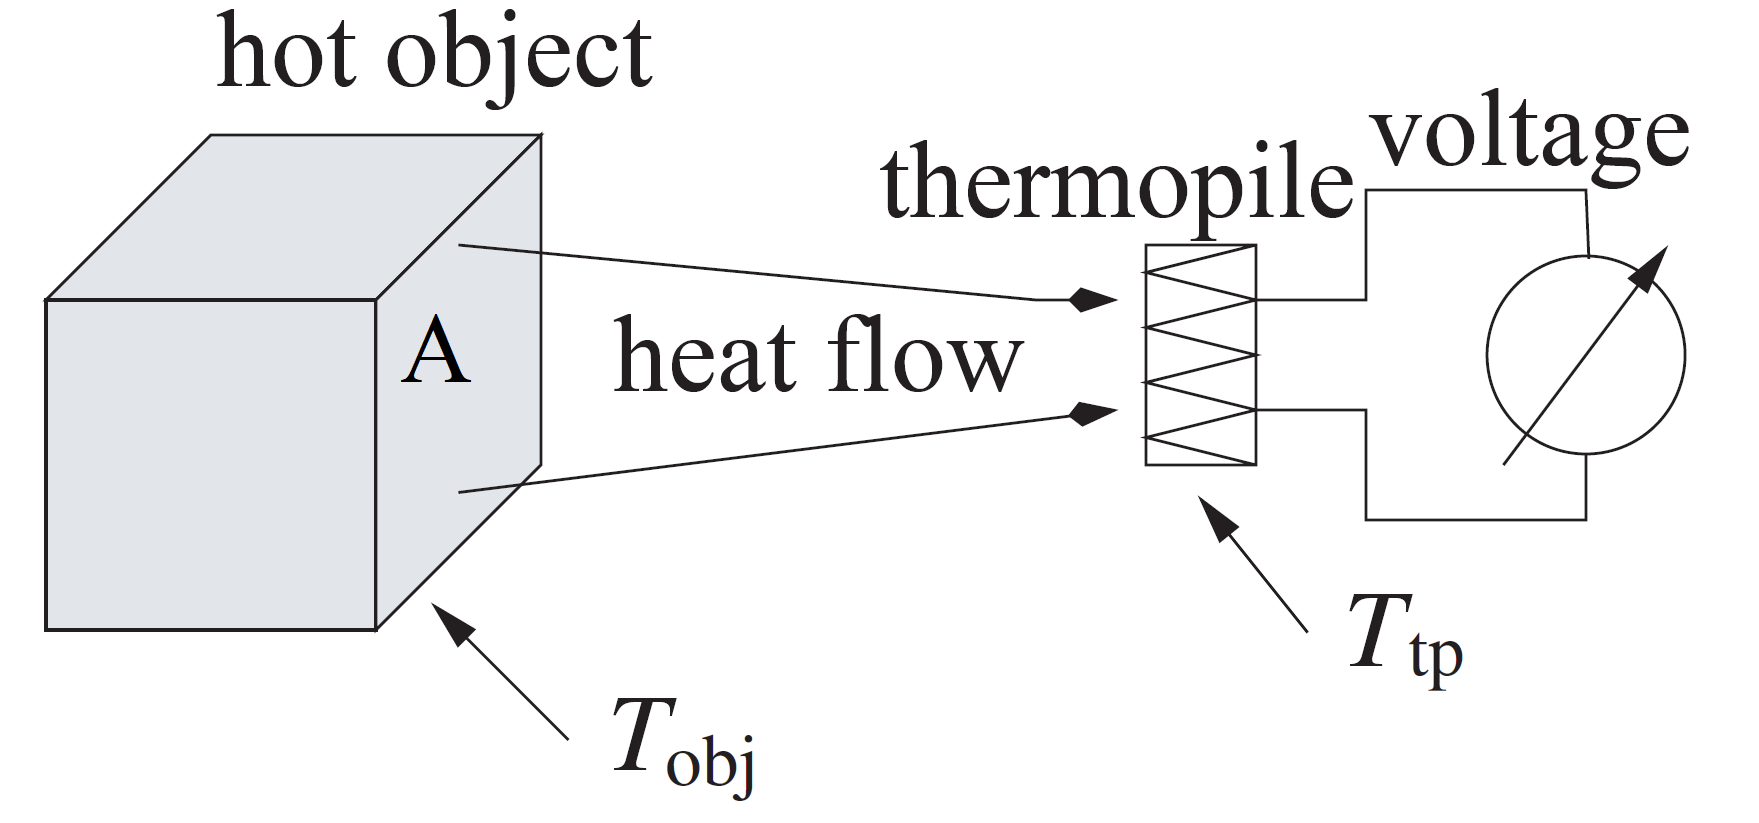
\includegraphics[width=0.5\textwidth]
	{fig/seebeck2.PNG}
	\caption[Aufbau Thermosäule]{Aufbau Thermosäule} \protect\cite{seebeck}
	\label{fig:thermosäule}
\end{figure}

Diese Formel zeigt auf, dass die Wärmestrahlung eines Körpers im wesentlichsten (mit 4. Potenz)
von der eigenen Temperatur abhängig ist. Die Fläche A ist lediglich proportional. Dies verursacht, dass bereits flächenmäßig kleine, jedoch stark erwärmte Objekte im Messbereich einen bedeutenden Einfluss auf die Messresultate liefern können. Zusätzlich Verursachen Wärmequellen im nahen Umfeld des Messbereichs Abweichungen auf die Messresultate.

Des Weiteren weist diese Formel auf eine weitere Problematik dieses Messprinzips hin, der mit dem Emissionsgrad $\epsilon$  in Verbindung steht. Der Emissionsgrad $\epsilon$ ist ein materialabhängiger, jedoch wellenlängenunabhängier Faktor, welcher zwischen 0-1 angegeben wird. Dieser gilt für graue Körper d.h. für Körper, dessen Oberfläche auftreffende Strahlung nicht vollständig absorbieren. Diese Eigenheit gilt für alle realen Körper. 

Nach dem Energieerhaltungsgesetz \protect\cite{Thermoformeln} gilt für Transmission, Reflexion und Absorption die Formel \ref{eq4}.
\begin{equation}
\label{eq4}
\tau  + \alpha + \varphi  = 1
\end{equation}
\myequations{Schwarzer Stahler, Energieerhaltung}

Wobei bei thermischen Gleichgewicht angenommen werden kann, dass der Emissionsgrad der Absortion entpsricht.

\begin{equation}
\label{eq5}
\epsilon \approx  \alpha
\end{equation}
\myequations{Strahlung Energieerhaltung Festkörper}


Da es sich Aufzügen nur von Festkörper ausgegangen wird, fällt die Transmission $\tau$ aus der Gleichung. Es können lediglich Reflexionen oder die Emission des Körpers Einfluss auf die einwirkende Infrarotstrahlung nehmen. Weitere Betrachtungen diesbezüglich werden im Unterkapitel 2.4. gemach

\section{geometrische Aspekte}
\label{sec:geometrie}

Da die Strahlungsintensität mit zunehmender Distanz mit zweiter Potenz abnimmt, spielt die Distanz zum Messobjekt eine entscheidende Rolle. Ein weiteres Kriterium ist der begrenzten \ac{FOV} des Sensors von 60$^\circ$. In der nachstehenden Skizze (Abbildung \ref{fig:Geometrie}) sind die Verhältnisse perspektivisch dargestellt. Dabei wird von einer Raumhöhe von 2.10 m ausgegangen. (nach Standardkabine EN 81-70)   

\begin{figure}[H]
	\centering
	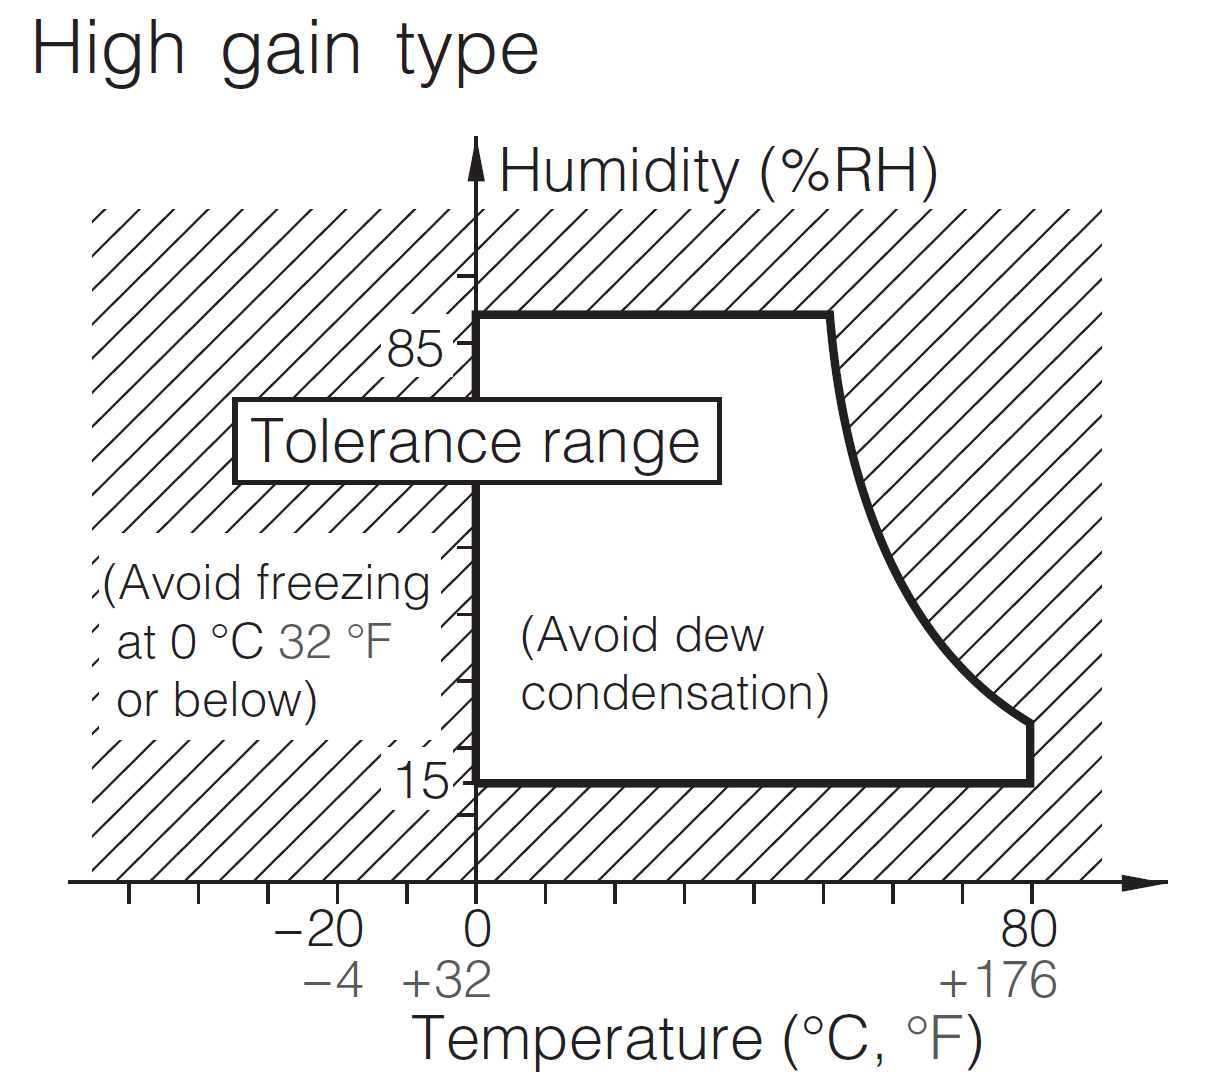
\includegraphics[width=0.5\textwidth]
	{fig/Humidity_Tolerance.PNG}
	\caption[Einfluss Luftfeuchtigkeit]{Einfluss Luftfeuchtigkeit} \protect\cite{AMG8834}
	\label{fig:Geometrie}
\end{figure}

Die räumliche Streckungen verursacht zusätzlich eine perspektivische Verzerrung, welcher in dieser Betrachtung nicht weiter beachtet wird. Zu sehen ist jedoch deutlich, dass bei der Messung von Personen die Messdistanz zwischen 10 bis 110 Zentimeter am relevantesten ist. In diesem Bereich kann jedoch mit dem aktuellen \ac{FOV} im besten Fall eine Fläche von 0.666 $ m/s^2 $ abgedeckt werden. Um eine Aufzugkabine mit 8 Personen\footnote[1]{Masse: (HxBxT) 2100 x 1100 x 1400 [mm]} bei mittlerem Messbereich wird im optimalen Fall ein Öffnungswinkel von 84°x 109°$^\circ$ benötigt. 

Problematisch kann in diesem Zusammenhang die Abschattung des Messbereichs durch grosse Personen sein, welche zentral positioniert sind. 

 

\section{Messobjekt und Messumgebung}
\label{sec:Messobjekt}
Dieses Kapitel beschreibt die Erkenntnisse bei der Betrachtung des Messobjekts und der Messumgebung. Dabei wurden einerseits die Kennwerte von Personen zusammengetragen, sowie die Messumgebung auf Störquellen und Einflussfaktoren begutachtet. Dank der Firma ARLEWO AG konnten unterschiedliche Aufzüge vermessen und bewertet werden. 

\subsection{Personen}
\label{subsec:Personen}

Die Reaktionen im menschlichen Körper sind auf eine Kerntemperatur von 37 °C. Am kältesten ist die Haut, die etwa 4 bis 7 Kelvin (Grad) kälter ist. Die Aufteilung der verschiedenen Arten der Wärmeabgabe beträgt bei einem ruhenden Menschen in einer Umgebung von 20 °C:


\begin{itemize}
	\item  46 \% Strahlung
	\item  33 \% Konvektion\footnote[2]{Konvektion bezeichnet die Wärmeabgabe an
		das umgebende Medium, in der Regel Luft}
	\item  19 \% Schwitzen
	\item   2 \% Atmung.
\end{itemize}

Die Höhe der Wärmeabgabe hängt im wesentlichen von der Schwere der Tätigkeit und von der Größe der Körperfläche ab. Daraus folgt, dass größere Personen mehr Wärme abgeben. Strahlung und Konvektion nehmen mit zunehmender Umgebungstemperatur bis zum Wert null bei 36 °C ab. Hat die Umgebung die Körpertemperatur erreicht, kann folglich durch Strahlung und Konvektion keine Wärme mehr abgeführt werden. In einer Umgebung mit Temperaturen oberhalb 37 °C kann also die Wärme nur noch durch Schwitzen abgeführt werden.\protect\cite{MenschWaerme}

\begin{figure}[H]
		\centering
	\begin{minipage}[b]{0.4\textwidth}
			\centering

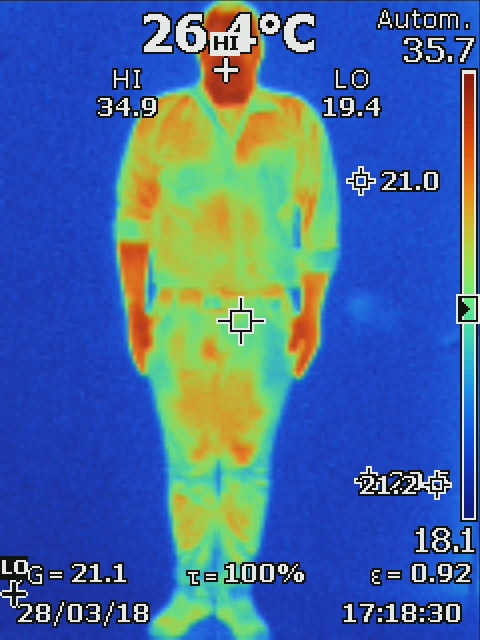
\includegraphics[width=0.8\textwidth]{fig/person_waerme.JPG}
\label{fig:Waermebild}
\caption[Wäermebild eines \\Probanden]{Wärmebild eines \\Probanden}
	\end{minipage}
	\begin{minipage}[b]{0.2\textwidth}
\end{minipage}
	\begin{minipage}[b]{0.4\textwidth}
			\centering
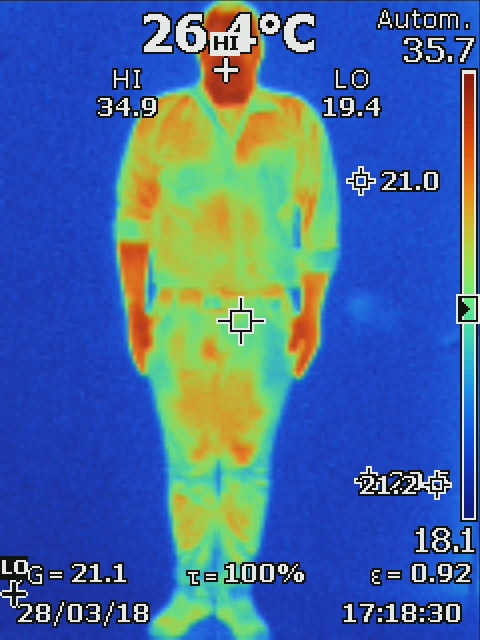
\includegraphics[width=0.8\textwidth]{fig/person_waerme.JPG}
\label{fig:Waermebild2}
\caption[Wäermebild eines \\Probanden]{Wärmebild eines \\Probanden}

	\end{minipage}
	
\end{figure}

Ein weiterer Aspekt, der sehr stark ins Gewicht fällt, ist die Art der Bekleidung. In Abbildung \ref{fig:Waermebild} und Abbildung \ref{fig:Waermebild2} ist deutlich zu sehen, dass das thermische Profil einer Person durch die Bekleidung stark variiert. Bekleidungsfreie Zonen n 

\subsection{Personenaufzüge}

In diesem Unterkapitel wurde der Personenaufzug als Messobjekt näher betrachtet. Neben räumlichen Parametern wie Höhe, Grundfläche und Volumen spielen vor allem die Oberflächenbeschaffenheit bzw. das Oberflächenmaterial Rolle. Weitere thermische Einflussfaktoren finden sich in der Umgebungstemperatur und der verbauten Leuchtmittel.


Wie bereits in \ref{sec:geometrie}

In Abbildung \ref{fig:Edelstahlgewalzt} und \ref{fig:Edelstahlmatt} sind 
\begin{figure}[H]
	\centering
	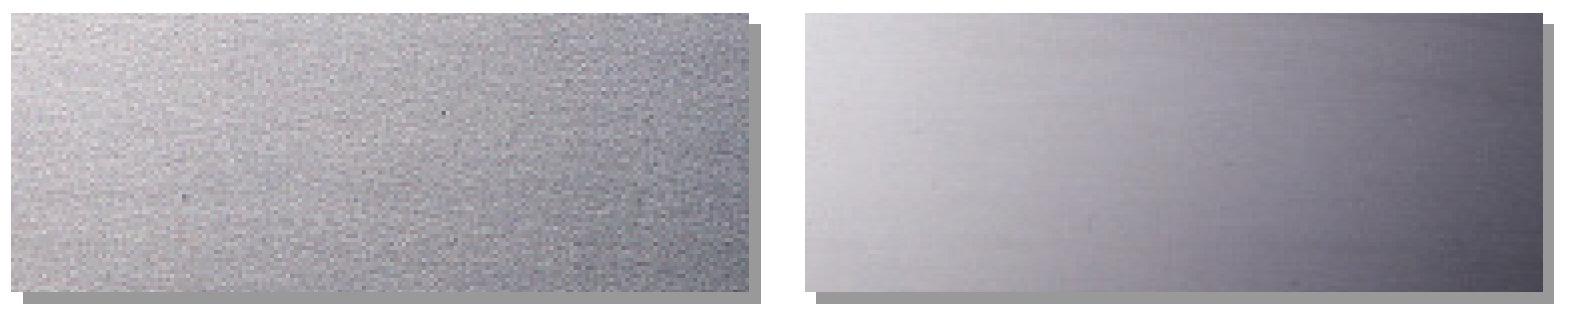
\includegraphics[width=0.8\textwidth]
	{fig/Edelstahl_gewalzt.PNG}
	\caption[Edelstahl warmgewalzt]{Edelstahl warmgewalzt} \protect\cite{Edelstahl}
	\label{fig:Edelstahlgewalzt}
\end{figure}
\begin{figure}[H]
	\centering
	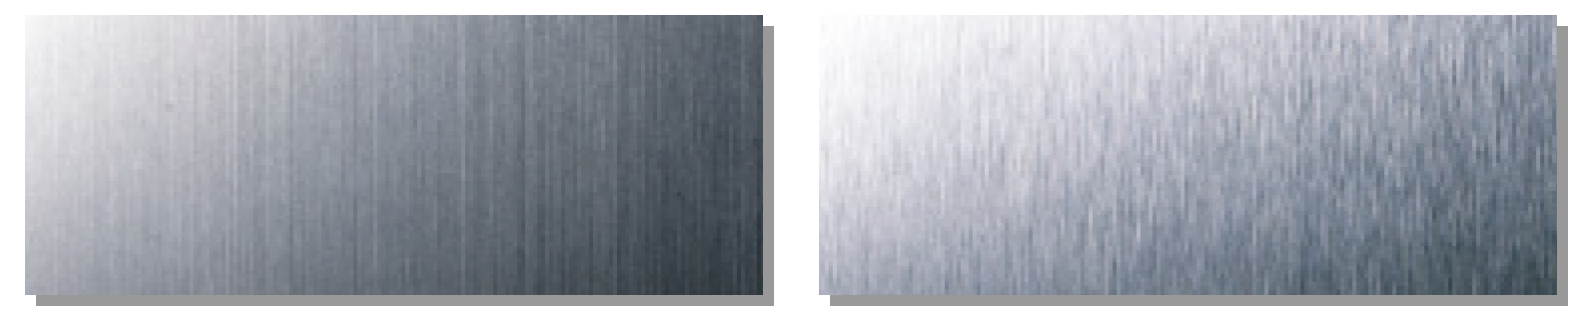
\includegraphics[width=0.8\textwidth]
	{fig/Edelstahl_matt.PNG}
	\caption[Edelstahl kaltgewalzt]{Edelstahl kaltgewalzt} \protect\cite{Edelstahl}
	\label{fig:Edelstahlmatt}	
\end{figure}




\begin{figure}[H]
	\centering
	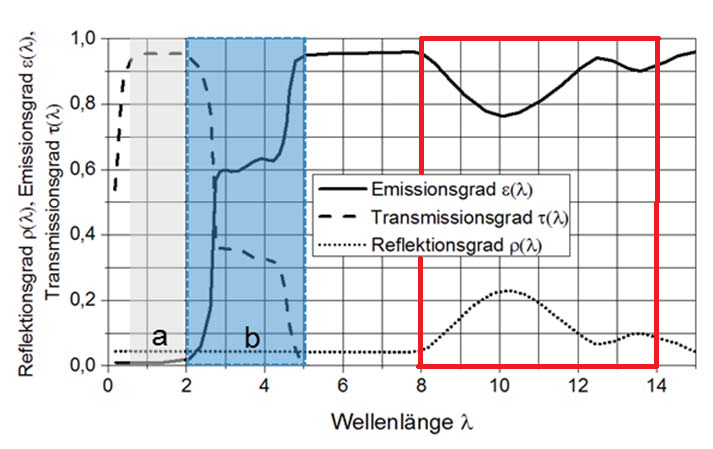
\includegraphics[width=0.8\textwidth]
	{fig/Glas_bearbeitet.png}
	\caption[Emissionsgrad in Abhängikeit zur Wellenlnge]{Emissionsgrad in Abhängikeit zur Wellenlnge} \protect\cite{Edelstahl}
	\label{fig:Glas}	
\end{figure}

\section{Fazit}

Die Personenerkennung in Aufzügen mit \ac{PIR} Sensoren ist am meisten von der Individualität einer Person abhängig. Faktoren wie Körpertemperatur, Körpergröße und Bekleidung verursachen enorme Differenzen. Dadurch kann kein einheitliches Profil erstellt werden. Der geometrische Aspekte Weitere physikalische Gegebenheiten wie die Umgebungstemperatur oder indirekte Sonneneinstrahlung bewirken veränderte Bedingungen für den Messbereich, welche bei einer Messeinheit berücksichtigt werden müssen.     




\chapter{Testphase 1}
\label{chap:Testphasen}

De

\section{Grundlagenmessungen}



\section{Streuung}


\section{Reflektion}


\section{Einfluss infrarotstrhlen}



\section{Personenmessungen}
















\section{Fazit}

\chapter{Personendetektion}
\label{chap:Personendetektion}


Dieser Abschnitt beschreibt das Vorgehen, um die Anzahl Personen in einem Aufzug zu erkennen. In einem ersten Schritt wird die Verarbeitung der Rohdaten aufgezeigt. Für den Auswertealgorithmus wurden mehrere unterschiedliche Aufzüge evaluiert und ein Profil erstellt. 



\begin{figure}[H]
	\centering
	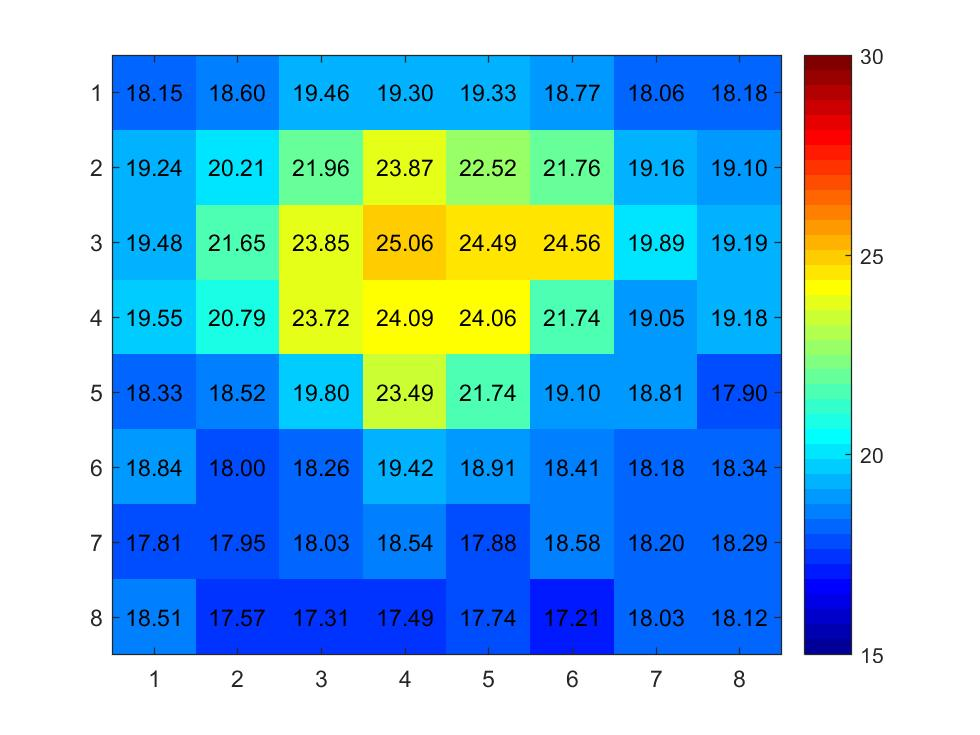
\includegraphics[width=0.5\textwidth]
	{fig/person_175_shirt.jpg}
	\caption[Pixeldarstellung einer Person]{Pxiedarstellung einer Person}
	\label{fig:Pixelbild}
\end{figure}



\section{Datenverarbeitung}




\section{Datenmanipulation mittels Interpolation}

Die Auflösung von 8x8 Pixel bietet optisch nur begrenzte Aussagekraft über die Anzahl Personen in einem Aufzug. Daher wurde mittels MATLAB mehrere Interpolationsverfahren benutzt, um die Auflösung der Personenerkennung zu verbessern. Im Zusammenhang mit den Pixelwerten eignet sich eine bikubische



Da im Zusammenhang mit dem Auswertealgorithmus mittels TensorFlow




\subsection{Profilbildung}


Im Verlauf der Arbeit wurden mehrere 


\section{Symetrische Erweiterung}



\section{Musterauswertung}




\section{Aufbau neuronales Netzwerk}

Convolutional Networks work by moving small filters across the input image. This means the filters are re-used for recognizing patterns throughout the entire input image. This makes the Convolutional Networks much more powerful than Fully-Connected networks with the same number of variables. This in turn makes the Convolutional Networks faster to train




The convolutional filters are initially chosen at random, so the classification is done randomly. The error between the predicted and true class of the input image is measured as the so-called cross-entropy. The optimizer then automatically propagates this error back through the Convolutional Network using the chain-rule of differentiation and updates the filter-weights so as to improve the classification error. This is done iteratively thousands of times until the classification error is sufficiently low.


(W -F +2P) : S+ 1

\section{Convolution Neural Network}


\begin{figure}[H]
	\centering
	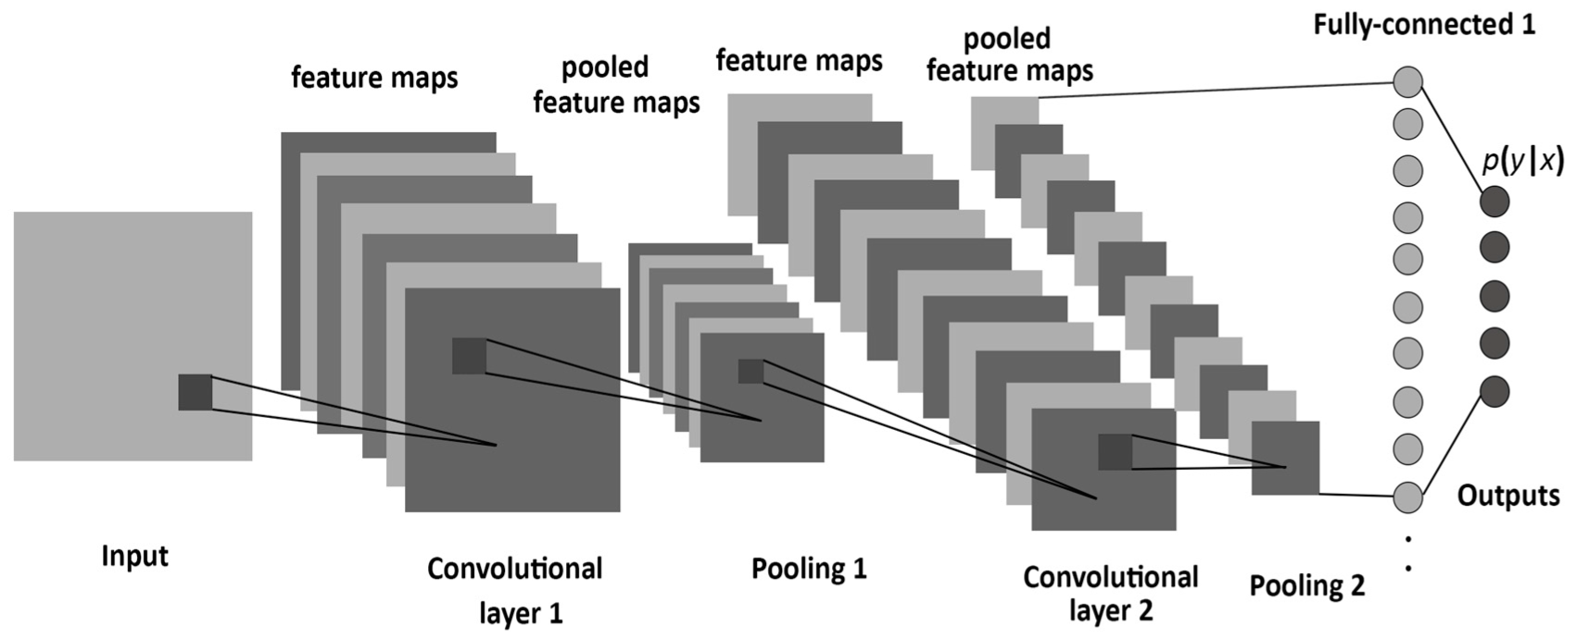
\includegraphics[width=1\textwidth]
	{fig/CCN.png}
	\caption[Aufbau des Convolutional Neural Network]{Aufbau des Convolutional Neural Network}
	\label{fig:CCN}
\end{figure}


Quelle: Computer Science and Engineering Department, University of Bridgeport, A Framework for Designing the Architectures of Deep Convolutional Neural Networks. Mai 2017, url:, http://www.mdpi.com/1099-4300/19/6?view=abstract&listby=pubdate_published+DESC%2Cfirstpage+DESC%2Cnumber+DESC&page_no=1 (besucht am 24.03. 2018).

\section{c}

Entweder alle Sekunde der Mittelwert auswerten, doer alle 100 ms die Daten auswerten 

\section{Fazit}



%Definition Umgebung
\newpage

\chapter{Empfehlung und Bewertung}
\label{Empfehlung_Vorgehen}

Dieses Kapitel beinhaltet eine Zusammenfassung der wichtigsten Erkenntnisse. Dabei werden die 


Bewertung von Auflösung
Bewertung von Geometrischen Aspekte
Bewertung Messprinzip

Bewertung von Personenerkennung

\section{Fazit}
\label{Fazit}


\section{Empfehlung}


Bewetungsraster


\section{Weiteres Vorgehen}


\section{Ausblick}

Diese Bachelorarbeit hat sich mit dem dem Panasonic Grid-Eye AMG8834 befasst. Während der Informationsbeschaffung wurde dieser mit erhältlichen Sensoren anderer Hersteller verglichen und als State-Of-The-Art beurteilt.  
Ab Mai 2018 wurde von der Firma Melexis der Sensor MLX90640 auf den Markt gebracht. Dieser Sensor könnte die Lücken, welche der verwendete Sensor besitzt schließen. Der MLX90640 besitzt mit einer Auflösung von 24x32 Pixel bedeutende Darstellung- und Auswertemöglichkeiten. Der Einsatztemperatur erstreckt sich zwischen -40$^\circ$ bis 85$^\circ$, daher ist er auch für extremere Umgebungstemperaturen geeignet. Interessant ist bei diesem Sensor das Model mit dem Öffnungswinkel von 110$^\circ$x75$^\circ$. Der Öffnungswinkel könnte die geometrische Problematik aus Kapitel \ref{sec:geometrie} lösen und somit für den Einsatzbereich in Personenaufzügen besser geignet sein. Preislich ist dieser Sensor jedoch doppelt so teuer wie der AMG8834. Das entsprechende Datenblatt ist im digitalen Anhang \ref{AnhangE} angefügt. 




\input{tex/Fazit}

\chapter{Reflexion}
\label{chap:Reflexion}

Dieses Kapitel beinhaltet neben den bedeutendsten Erläuterungen zum Projektmanagement auch ein persönliches Resümee im Schlusswort. Mit den entsprechenden Danksagung an alle Personen, welche mich bei dieser Arbeit unterstützt haben, endet der inhaltliche Teil.


\section{Erläuterungen zum Projektmanagement}
\label{Projektmanagement}
Im Rahmen dieser Arbeit wurden anfänglich die Meilensteine definiert und ein Risikomanagement erstellt. Da diverse Meilensteine voneinander abhängig sind, mussten im Verlauf der Arbeit diese angepasst werden. In Anhang \ref{AnhangA} und \ref{AnhangC} ist der Meilensteinplan V3 und das Risikomanagement angefügt.

Neben der Planung wurden die wöchentlichen Besprechungen protokolliert und entsprechende Erkenntnisse in die Planung miteinbezogen. 

Der detaillierte Projektplan V3 im Anhang \ref{AnhangB} bietet vollständigen Überblick über die erledigten Tätigkeiten während der gesamten Arbeit. Dabei sind die Meilensteine \textcolor{darkgray}{grau} markiert.

Es wurde ein SCRUM ähnliches Verfahren angewendet, um alle anstehenden Aufgaben systematisch abzuarbeiten. Der detaillierte Projektplan gibt zudem auch den geschätzten und effektiven Zeitaufwand der Tätigkeit wieder.

Der gesamthaft, berechnete Zeitaufwand ist in der Tabelle  \ref{tab:Zeitaufwand} dargestellt. Die entstandenen Differenz des Soll-Ist-Vergleich wird in nachfolgenden Abschnitt erläutert.

\begin{table}[H]
	\centering
	\caption{Soll-Ist-Vergleich zeitlicher Aufwendungen in [h]}
	\begin{tabular}{|c|c|c|}
		\hline
		\rowcolor[HTML]{9B9B9B} 
	\multicolumn{1}{|c|}{\cellcolor[HTML]{9B9B9B}\textbf{Soll-Aufwand}} &  \multicolumn{1}{c|}{\cellcolor[HTML]{9B9B9B}{\color[HTML]{333333} \textbf{Ist-Aufwand}}} & \textbf{zeitliche Differenz} \\ \hline
		420.5
		& 472.25                                                                                           &    
		52.25                \\ \hline
	\end{tabular}
	\label{tab:Zeitaufwand}
\end{table}

Im allgemeinen wurde die Aufwände der einzelnen Tätigkeiten eher unterschätzt. Dabei sind vor allem die Zeitdifferenzen der Projektphasen; Hardware/Software V1, Datenerfassung \& Auswertung TP1 und die Dokumentation ausschlaggebend für die Differenz.

Für die Informationsbeschaffung musste mehr Zeit aufgewendet werden, bis die Grundlagen des Messprinzips verstanden wurden. Daher wurde der Zeitraum verlängert.

Der Testaufbau und die Durchführungen benötigen enorm viel Zeit, da jede Messung vor- und nachbearbeitet wurde. Dabei nehmen die Parameteridentifikation und die Auswertung der Messergebnisse zusätzliche Zeit in Anspruch. 

Die Softwareimplementierung des \ac{CNN} war bedeutend aufwendiger als angenommen. Viele kleine Fehler verursachten Verzögerungen, daher musste dieser Projektabschnitt um eine Woche verlängert werden. 

Es wurde noch Zeit aufgewendet eine Echtzeitmesseinheit zu erstellen. Diese Messeinheit war in der anfänglichen Planung nicht enthalten. 

Ansonsten konnten die geschätzten zeitlichen Rahmen eingehalten werden. Für die gesamte Projektplanung sowie der Aktualisierungen des Zeitplans und der Tätigkeiten wurde eine aufsummierte







\newpage
\section{Schlusswort}

Mit der zunehmenden Verbreitung von Internet of Things in alltäglichen Situation bieten simple Sensoren neue Anwendungsmöglichkeiten. Das Potential von neuronalen Netzwerken für die Bilderkennung zeigen Vorzeigeprojekte wie das \acsfont{MNIST Dataset}. Auch in der thermografischen Bilderkennung bietet dieses Modellierungsverfahren Ansätze.

Da keine persönlichen Grundkenntnisse in diesem Themengebiet vorgängig vorhanden war, war der Einstig in dieses Thema anfänglich zeitraubend. Dennoch konnte durch gute Literaturen und Unterstützung an der Hochschule Luzern entsprechende Kenntnisse erworben werden. 

dbietet diese Bachelorarbeit ein breites Spektrum an Know-How um die vorgegebene Aufgabenstellung zu lösen.

Abschliessend ist noch zu erwähnen, dass   Gerade der Bereich der intelligenten Systemen zukünftig ein mehr und mehr zentraleres Thema für angehende Elektroingenieure wird. Daher ist es erfreulich, dass gerade solche Aufgaben in Zusammenarbeit mit Industriepartnern an der Hochschule Luzern in Angriff genommen werden.



  



\section{Danksagung}

An dieser Stelle möchte ich mich bei allen bedanken, die mich bei der Ausführung dieser
Arbeit unterstützt haben. 
Zuallererst gebührt der Dank an Kilian Schuster, der mich als betreuender Dozent bei dieser Bachelorarbeit tatkräftige unterstützt hat, sowie mit wertvollen Hinweisen und ehrlichen Rückmeldungen zur Seite gestanden ist. Mein Dank geht auch an Manuel Serquet, der mich mt TensorFlow vertraut gemacht hat und einige Unklarheiten klären konnte. 

Ebenfalls bedanken ich mich bei den Gegenlesern Julia Schuler und Marie-Theres Zimmermann für die syntaktische und inhaltliche Korrektur der wissenschaftlichen Dokumentation.

Ein speziellen Dank geht an die Immobilienverwaltungsfirma ARLEWO in Stans, welche mir ein breites Spektrum an Schindler Aufzügen bereitstellte, damit die Feldmessungen praxisnahe durchgeführt werden konnten. An diesem Punkt besten Dank auch allen Probanden, welche sich für die Feldmessungen zur Verfügung gestellt haben.

%Freigabe des Ind. Partners und Dozent
\newpage


%Inhalt Anhang
\appendix

\chapter{Aufgabenstellung}
\label{AnhangAufgabenstellung}

Die Aufgabenstellung wurde im Februar 2018 übergeben und beinhaltet neben der Erläuterung der Aufgabe, weitere Anforderungen und Termine.

Dieses Dokument ist auch im digitalen Anhang \ref{AnhangDig} einsehbar.

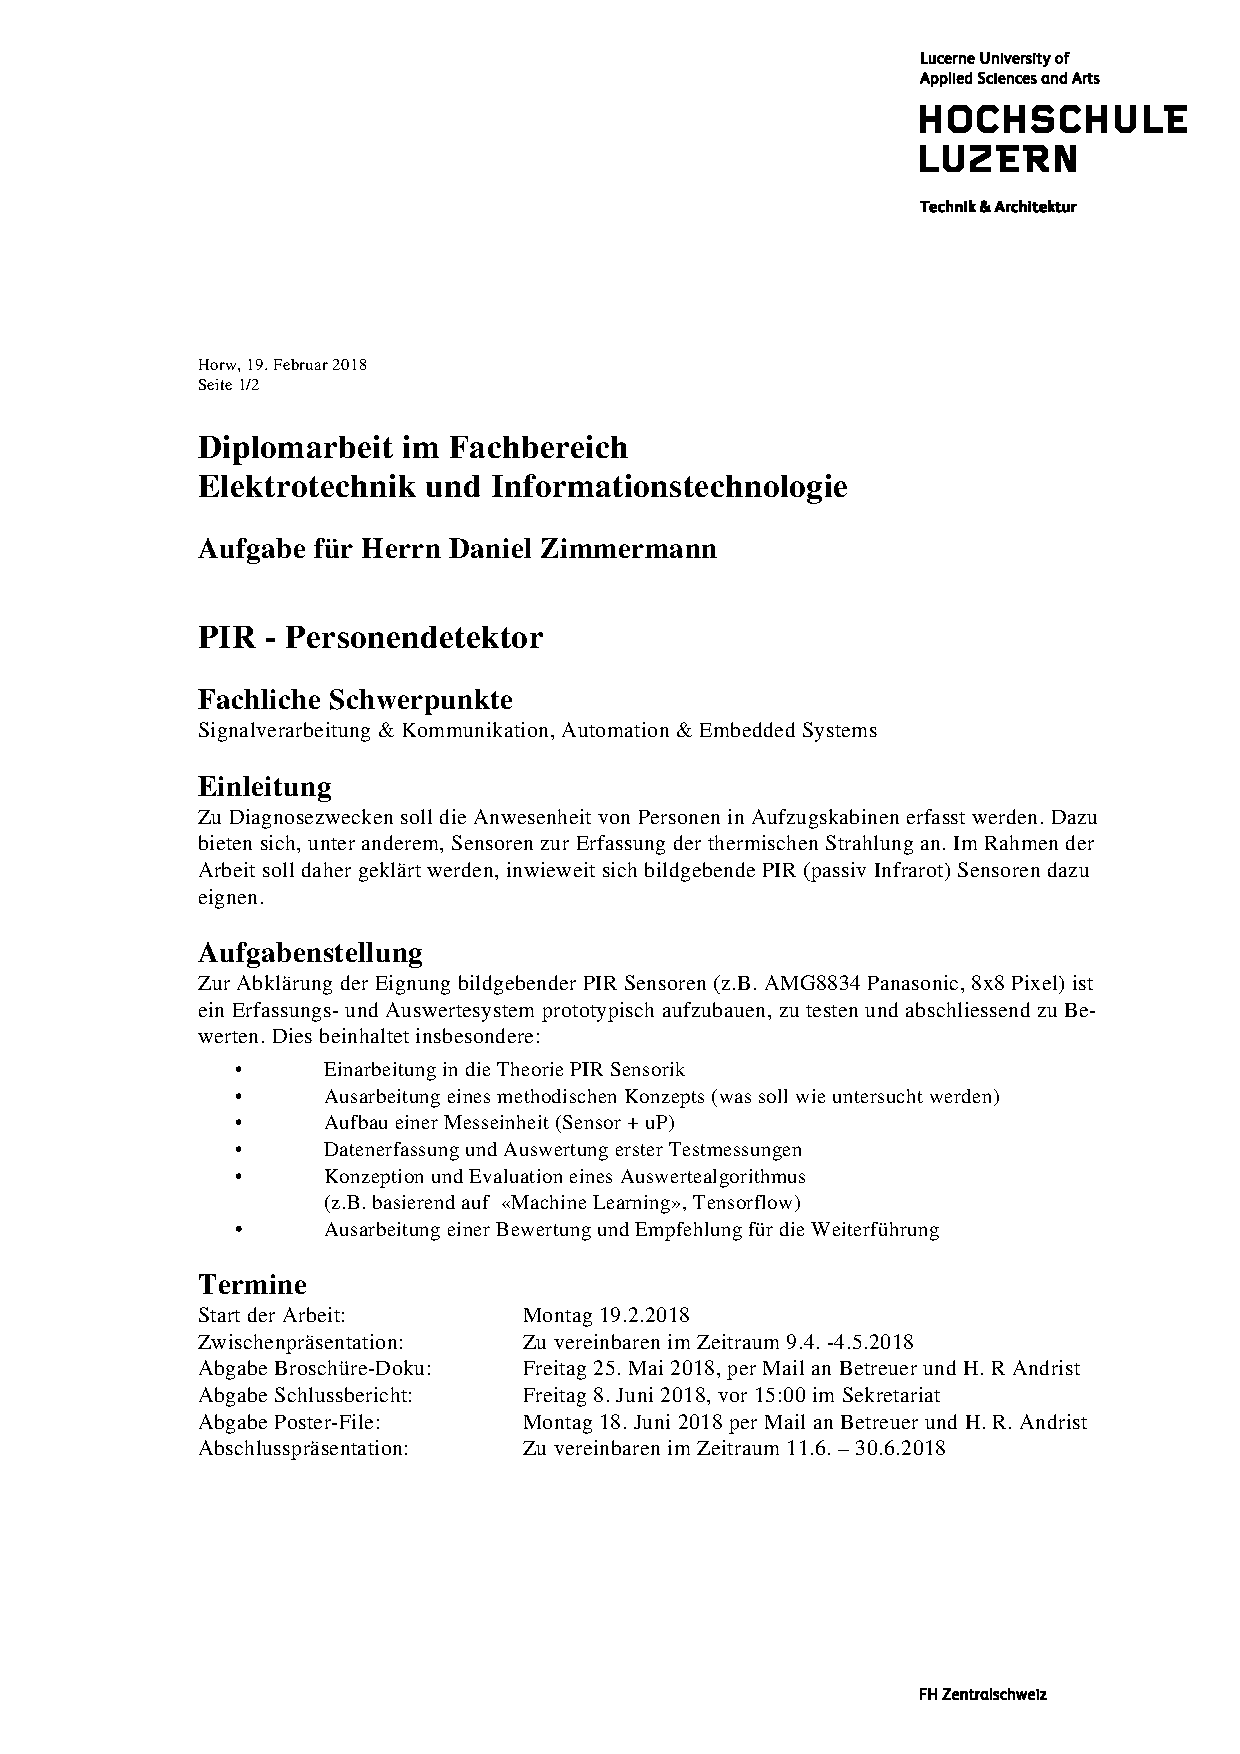
\includepdf[pages=-]{Anhang/Aufgabenstellung.pdf}

\chapter{Meilensteinplan}
Der Meilensteinplan wurde in der Initialisierungsphase erstellt und während dem Projektablauf angepasst. Die Meilensteine wurden farblich unterteilt. Die Unterteilungen sind in der Legende beschrieben. 

Dieses Dokument ist auch im digitalen Anhang \ref{AnhangDig} einsehbar.

\label{AnhangA}
\includepdf[pages=1,angle=90]{Anhang/Meilensteinplan_BAT_P1_V3.pdf}

\chapter{Detaillierter Projektplan}
\label{AnhangB}

Der detaillierte Projektplan gibt alle wesentlichen Tätigkeiten während des gesamten Projekt wieder. Dabei sind die Projektabschnitte und die Meilensteine angegeben.

Der Projektplan wurde für eine bessere Übersicht in zwei Teile unterteilt. 
\begin{itemize}
\item Der erste Teil ist der Zeitraum von der Initialisierung bis zur Zwischenpräsentation.

\item Der zweite Teil ist der Zeitraum von der Zwischenpräsentation bis zur Projektbeendigung.

\end{itemize}

Die einzelnen Tätigkeiten wurden auf zeitliche Aufwendungen geschätzt und der effektive Aufwand wird als Soll-Ist-Vergleich angegeben. 
Jedem Projektabschnitt werden die Zeitaufwendungen separat angerechnet. In jedem Teil ist in \textcolor{yellow}{gelber} Markierung die gesamthafte zeitliche Aufwendung angegeben.


Dieses Dokument ist auch im digitalen Anhang \ref{AnhangDig} einsehbar.


%\includepdf[pages=1,angle=90]{Anhang/01_Detaillierter Projektplan BAT V3.pdf}

%\includepdf[pages=1,angle=90]{Anhang/02_Detaillierter Projektplan BAT V3.pdf}



\chapter{Risikomanagement}
\label{AnhangC}
\setcounter{page}{9}
Das Risikomanagement wurde in der Initialisierungsphase erstellt und gibt Auskunft, welche Risiken bei dieser Arbeit zu beachten sind.

Eine Bewertung der Wahrscheinlichkeiten und den Auswirkungen gibt Auskunft, welche Risiken vorrangig beachtet werden müssen.  Dabei wurden diese in Standardrisiken und Projektbezogene Risiken unterteilt.

Dieses Dokument ist auch im digitalen Anhang \ref{AnhangDig} einsehbar.

\includepdf[pages=-,angle=90]{Anhang/Risikomanagement_V2.pdf}
\chapter{Übersicht Aufzugsprofile }
\label{AnhangD}

Es werden nachfolgend die drei verschiedenen Aufzugsprofile abgebildet. Dabei werden die wichtigsten Eigenschaften der erstellten Profile dargelegt. Daneben werde die Messpositionen, der verschiedenen Personenmessung mit den Buchstaben aus Unterkapitel \ref{subsec:Personen} angegeben. Die Buchstaben K, M und G stehen für die Probandengrössen; klein, mittel und gross, welche auch in  Unterkapitel \ref{subsec:Personen} erläutert sind.
\newpage


\section{Profil 1}
Beim Profil 1 handelt es sich um einem mittelgrossen Aufzug. Die Messungen wurde am 28.03.2018 am Messort Stansstad Bahnhofstrasse erstellt. Der Aufzugs mit der Kommissionsnummer 11018490 ist vom Baujahr 2017.
 


		\begin{figure}[!ht]
	\centering
	\begin{minipage}[b]{0.3\linewidth}
		\centering
		\includegraphics[width=0.9\linewidth]{fig/Gesamt1.jpeg}
		\caption{Gesamtbild}
		\label{fig:profilAnhang1}
	\end{minipage}
	\begin{minipage}[b]{0.3\linewidth}
		\centering
		\includegraphics[angle=270, width=0.9\linewidth]{fig/Raster1.jpg}
		\caption{Messraster}
		\label{fig:profilAnhang2}
	\end{minipage}
	\begin{minipage}[b]{0.3\linewidth}
		\centering
		\includegraphics[width=0.9\linewidth]{fig/beleuchtung1.jpeg}
		\caption{Beleuchtung}
		\label{fig:profilAnhang3}
	\end{minipage}
\end{figure}

\begin{table}[H]
	\centering
	\caption{Aufzugseigenschaften Profil 1}
	\label{aufzug1}
	\begin{tabular}{|c|c|c|c|c|c|}
		\hline
		\rowcolor[HTML]{9B9B9B} 
		\cellcolor[HTML]{9B9B9B}{\color[HTML]{333333} }                                                                                             & {\color[HTML]{333333} \textbf{Breite {[}m{]}}} & {\color[HTML]{333333} \textbf{Höhe {[}m{]}}} & {\color[HTML]{333333} \textbf{Tiefe {[}m{]}}} & \textbf{Bodenfäche  {[}$m^2${]}} & \textbf{Auslegung  } \\ \cline{2-6} 
		\multirow{-2}{*}{\cellcolor[HTML]{9B9B9B}{\color[HTML]{333333} \textbf{\begin{tabular}[c]{@{}c@{}}Aufzugs-\\ eigenschaften\end{tabular}}}} & 1.105                                          & 2.127                                        & 1.401                                         & 1.548                            & 8 Pers.                \\ \hline
		\rowcolor[HTML]{9B9B9B} 
		\cellcolor[HTML]{9B9B9B}                                                                                                                    & \textbf{Decke}                                 & \textbf{Boden}                               & \textbf{Front}                                & \textbf{Seitenwände}             & \textbf{Beleuchtung}       \\ \cline{2-6} 
		\multirow{-2}{*}{\cellcolor[HTML]{9B9B9B}\textbf{Materialaufbau}}                                                                           & Edelstahl                                      & Gummi                                        & Edelstahl                                     & Laminat                          & LED Strips                 \\ \hline
	\end{tabular}
\end{table}

\begin{table}[H]
	\centering
	\caption{Temperaturwerte Profil 1}
	\label{temp1}
	\begin{tabular}{|c|c|c|c|}
		\hline
		\rowcolor[HTML]{9B9B9B} 
		\cellcolor[HTML]{9B9B9B}{\color[HTML]{333333} }                                                                                                   & {\color[HTML]{333333} \textbf{Aussentemp. Aufzug}} & {\color[HTML]{333333} \textbf{Innentemp. Aufzug}} & {\color[HTML]{333333} \textbf{Oberflächentemp.}} \\ \cline{2-4} 
		\multirow{-2}{*}{\cellcolor[HTML]{9B9B9B}{\color[HTML]{333333} \textbf{\begin{tabular}[c]{@{}c@{}}Temperatur\\ Messdaten in °C\end{tabular}}}} & 19.9                                               & 20.1                                              & 16.5                                             \\ \hline
	\end{tabular}
\end{table}

 \textbf{Messpositionen:}\\
\textbf{1. Person Kat. K:} A, B, D, E, G, I, J\\
\textbf{1. Person Kat. G:} A, B, D, E, G, I, J\\
\textbf{2. Person Kat. K,G:} AB, AC, AI, DE, DF, GC, JE, JI  \\
\textbf{2. Person Kat. M,G:} AB, AC, AI, DE, DF, GC, JE, JI  \\
\textbf{3. Person Kat. K,M,G:} AEI, ABC, IEA, GEI, GKI, HDI, JHL \\
\textbf{4. Person Kat, K,K,M,G:} ACDF, CAFD, ACJL, ADGJ, DFGI, GJCF \\
\textbf{Trainingsetgrösse:}         151936 Frames \\
	
	\newpage
	
	
	\section{Profil 2}
Beim Profil 2 handelt es sich um einen grossen Aufzug. Die Messungen wurde am 10.05.2018 am Messort Wolfenschiessen Hauptstrasse erstellt. Der Aufzugs mit der Kommissionsnummer 20052781 ist vom Baujahr 2018.

	
	
		\begin{figure}[!ht]
	\centering
	\begin{minipage}[b]{0.3\linewidth}
		\centering
		\includegraphics[angle=270, width=0.9\linewidth]{fig/Gesamt2.jpg}
		\caption{Gesamtbild}
		\label{fig:profilAnhang4}
	\end{minipage}
	\begin{minipage}[b]{0.3\linewidth}
		\centering
		\includegraphics[angle=270,width=0.9\linewidth]{fig/Raster2.jpg}
		\caption{Messraster}
		\label{fig:profilAnhang5}
	\end{minipage}
	\begin{minipage}[b]{0.3\linewidth}
		\centering
		\includegraphics[angle=180,width=0.9\linewidth]{fig/beleuchtung2.jpg}
		\caption{Beleuchtung}
		\label{fig:profilAnhang6}
	\end{minipage}
\end{figure}

\begin{table}[H]
	\centering
	\caption{Aufzugseigenschaften Profil 2}
	\label{aufzug2}
	\begin{tabular}{|c|c|c|c|c|c|}
		\hline
		\rowcolor[HTML]{9B9B9B} 
		\cellcolor[HTML]{9B9B9B}{\color[HTML]{333333} }                                                                                             & {\color[HTML]{333333} \textbf{Breite {[}m{]}}} & {\color[HTML]{333333} \textbf{Höhe {[}m{]}}} & {\color[HTML]{333333} \textbf{Tiefe {[}m{]}}} & \textbf{Bodenfäche  {[}$m^2${]}} & \textbf{Auslegung  } \\ \cline{2-6} 
		\multirow{-2}{*}{\cellcolor[HTML]{9B9B9B}{\color[HTML]{333333} \textbf{\begin{tabular}[c]{@{}c@{}}Aufzugs-\\ eigenschaften\end{tabular}}}} & 1.560                                          & 2.105                                        & 2.031                                         & 3.168                            & 20 Pers.                \\ \hline
		\rowcolor[HTML]{9B9B9B} 
		\cellcolor[HTML]{9B9B9B}                                                                                                                    & \textbf{Decke}                                 & \textbf{Boden}                               & \textbf{Front}                                & \textbf{Seitenwände}             & \textbf{Beleuchtung}       \\ \cline{2-6} 
		\multirow{-2}{*}{\cellcolor[HTML]{9B9B9B}\textbf{Materialaufbau}}                                                                           & Edelstahl                                      & Granit                                        & Edelstahl                                     & Edelstahl                          & LED Spots                 \\ \hline
	\end{tabular}
\end{table}

\begin{table}[H]
	\centering
	\caption{Temperaturwerte Profil 2}
	\label{temp2}
	\begin{tabular}{|c|c|c|c|}
		\hline
		\rowcolor[HTML]{9B9B9B} 
		\cellcolor[HTML]{9B9B9B}{\color[HTML]{333333} }                                                                                                   & {\color[HTML]{333333} \textbf{Aussentemp. Aufzug}} & {\color[HTML]{333333} \textbf{Innentemp. Aufzug}} & {\color[HTML]{333333} \textbf{Oberflächentemp.}} \\ \cline{2-4} 
		\multirow{-2}{*}{\cellcolor[HTML]{9B9B9B}{\color[HTML]{333333} \textbf{\begin{tabular}[c]{@{}c@{}}Temperatur\\ Messdaten in °C\end{tabular}}}} & 22.2                                               & 22.5                                              & 19.7                                             \\ \hline
	\end{tabular}
\end{table}

 \textbf{Messpositionen:}\\
\textbf{1. Person Kat. K:} A, B, D, E, G, I, J\\
\textbf{1. Person Kat. G:} A, B, D, E, G, I, J\\
\textbf{2. Person Kat. K,G:} AB, AC, AI, DE, DF, GC, JE, JI   \\
\textbf{2. Person Kat. K,M:} AB, AC, AI, DE, DF, GC, JE, JI   \\
\textbf{3. Person Kat. K,M,K:} AEI, ABC, IEA, GEI, GKI, HDI, JHL \\
\textbf{4. Person Kat, K,K,M,G:} ACDF, CAFD, ACJL, ADGJ, DFGI, GJCF \\
\textbf{Trainingssetgrösse:} 153181 Frames


	\newpage
\section{Profil 3}
Beim Profil 3 handelt es sich um einen kleine Aufzug. Die Messungen wurde am 12.05.2018 am Messort Stansstad Dorfstrasse erstellt. Der Aufzugs mit der Kommissionsnummer 54004012294 ist vom Baujahr 1988.

		
		\begin{figure}[!ht]
	\centering
	\begin{minipage}[b]{0.3\linewidth}
		\centering
		\includegraphics[angle=270,width=0.9\linewidth]{fig/Gesamt3.jpg}
		\caption{Gesamtbild}
		\label{fig:profilAnhang7}
	\end{minipage}
	\begin{minipage}[b]{0.3\linewidth}
		\centering
		\includegraphics[angle=270,width=0.9\linewidth]{fig/Raster3.jpg}
		\caption{Messraster}
		\label{fig:profilAnhang8}
	\end{minipage}
	\begin{minipage}[b]{0.3\linewidth}
		\centering
		\includegraphics[angle=180,width=0.9\linewidth]{fig/beleuchtung3.jpg}
		\caption{Beleuchtung}
		\label{fig:profilAnhang9}
	\end{minipage}
\end{figure}

\begin{table}[H]
	\centering
	\caption{Aufzugseigenschaften Profil 3}
	\label{aufzug1}
	\begin{tabular}{|c|c|c|c|c|c|}
		\hline
		\rowcolor[HTML]{9B9B9B} 
		\cellcolor[HTML]{9B9B9B}{\color[HTML]{333333} }                                                                                             & {\color[HTML]{333333} \textbf{Breite {[}m{]}}} & {\color[HTML]{333333} \textbf{Höhe {[}m{]}}} & {\color[HTML]{333333} \textbf{Tiefe {[}m{]}}} & \textbf{Bodenfäche  {[}$m^2${]}} & \textbf{Auslegung  } \\ \cline{2-6} 
		\multirow{-2}{*}{\cellcolor[HTML]{9B9B9B}{\color[HTML]{333333} \textbf{\begin{tabular}[c]{@{}c@{}}Aufzugs-\\ eigenschaften\end{tabular}}}} & 1.095                                          & 2.105                                        & 1.246                                         & 1.364                            & 6  Pers.                \\ \hline
		\rowcolor[HTML]{9B9B9B} 
		\cellcolor[HTML]{9B9B9B}                                                                                                                    & \textbf{Decke}                                 & \textbf{Boden}                               & \textbf{Front}                                & \textbf{Seitenwände}             & \textbf{Beleuchtung}       \\ \cline{2-6} 
		\multirow{-2}{*}{\cellcolor[HTML]{9B9B9B}\textbf{Materialaufbau}}                                                                           & Edelstahl                                      & Granit                                       & Edelstahl                                     & Kunststoff                         & Leuchtstoff                 \\ \hline
	\end{tabular}
\end{table}

\begin{table}[H]
	\centering
	\caption{Temperaturwerte Profil 3}
	\label{temp3}
	\begin{tabular}{|c|c|c|c|}
		\hline
		\rowcolor[HTML]{9B9B9B} 
		\cellcolor[HTML]{9B9B9B}{\color[HTML]{333333} }                                                                                                   & {\color[HTML]{333333} \textbf{Aussentemp. Aufzug}} & {\color[HTML]{333333} \textbf{Innentemp. Aufzug}} & {\color[HTML]{333333} \textbf{Oberflächentemp.}} \\ \cline{2-4} 
		\multirow{-2}{*}{\cellcolor[HTML]{9B9B9B}{\color[HTML]{333333} \textbf{\begin{tabular}[c]{@{}c@{}}Temperatur\\ Messdaten in °C\end{tabular}}}} & 17.5                                               & 17.7                                              & 17.5                                             \\ \hline
	\end{tabular}
\end{table}

 \textbf{Messpositionen:}\\
\textbf{1. Person Kat. K:} A, B, D, E, G, I, J\\
\textbf{1. Person Kat. G:} A, B, D, E, G, I, J\\
\textbf{2. Person Kat. K,K:} AB, AC, AI, DE, DF, GC, JE, JI   \\
\textbf{2. Person Kat. K,G:} AB, AC, AI, DE, DF, GC, JE, JI   \\
\textbf{3. Person Kat. K,G,K:} AEI, ABC, DEF, ABI, DHL, GEI, GKI, HDC \\
\textbf{4. Person Kat K,K,M,G:} ACDF, ACJL, ADGI, DFAC, DFGI, GJCF \\
\textbf{Trainingsetgrösse:}         154461 Frames \\			
			
		\chapter{Emissionsgradtabelle}
			\label{AnhangE}
			
			Die Emissionsgrade von Materialien variieren, daher wurde zur Übersicht eine entsprechende Emissionsgradtabelle angefügt. Die Emissionsgradtabelle wurde aus der Literatur von \cite{Thermoformeln} entnommen.
			
			
			
\includepdf[pages=-]{Anhang/emissionsgradtabelle.pdf}
			
			
			\chapter{Digitale Projektanhänge}
			\label{AnhangDig}
			
			Der digitale Projektanhang innen auf der Rückseite des Berichts enthält neben dem Schlussbericht und dem Projektmanagement,alle Datenblätter, Rohdaten und Programme in strukturierter Form. Alle Matlab- und Python-Programme sind kommentiert und geben Auskunft über die Funktionen. Die Unterordner enthalten "readme" Textfiles, die zusätzliche Informationen bieten.
			
			\section{Ordnerstruktur CD}
			
			
			Die beiliegende CD hat folgende Ordnerstruktur.
			
			\begin{enumerate}
				\item Abgabedokument
				\begin{itemize}
					\item BAT\_Schlussdokumentation.pdf
				\end{itemize}
				\item Projektmanagement
				\begin{itemize}
					\item Aufgabenstellung
					\item Meilensteinplan P2 V3
					\item Detaillierter Projektplan V3 Teil 1 \& 2
					\item Risikomanagement V3
					\item Besprechungsprotokolle
					\item Bestellungen
				\end{itemize}
				\item Testdurchführungen
				\begin{itemize}
					\item Testkonzepte \& Testmappen
					\item Matlab Messungen \& Skripts
				\end{itemize}
				\item Messdaten
				\begin{itemize}
					\item Testkonzepte \& Testmappen
					\item H-Term 
					\item ConvertValue\_V2
				\end{itemize}
				\item Software Personenerkennung
				\begin{itemize}
					\item Personendetection\_Modelling\_V3\_ProfilX.py
					\item input\_data.py
					\item rawDataMergeV3\_ProfilX.py
					\item rotate\_and\_swap\_ProfilX.py
					\item Modelle
					\item Datensätze
				\end{itemize}
				\item Profile
				\begin{itemize}
					\item Profile 1
					\item Profile 2
					\item Profile 3
					\item Testprofile 	
					\item Gesamtprofil	
				\end{itemize}
				\item Datenblätter
				\begin{itemize}
					\item Panasonic AMG8834
					\item Melexis MLX90640
					\item Fluke TI-52-II
					\item Fluke TI 125 
				\end{itemize}
			\end{enumerate}
			
			\newpage
			

				

